Multiple choice section. All points are for choosing the correct answer. No justification is needed.
\begin{questions} 




\question[3] When is a graph not the graph of a function?
\begin{checkboxes}
    \choice When the graph is a straight line.
    \choice When at least one vertical line intersects the graph at more than one point.
    \choice When the graph goes off to infinity.
    \choice When there is at least one vertical line that does not intersect the graph.
    \choice None of the above.
\end{checkboxes}

\question[3] Select the correct graph of $f(x)=\left\{\begin{matrix}
    x^2 &,& x\ge 0\\
    -x &,& x<0
\end{matrix}\right.$  
\begin{multicols}{2}
    

\begin{checkboxes}
    \choice \phantom{a}\vspace{-.7cm}
    
    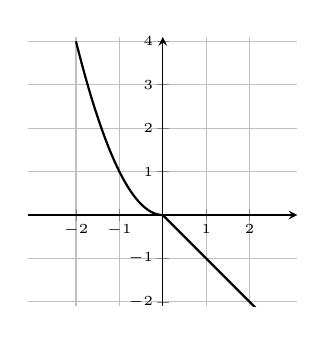
\begin{tikzpicture}%[domain=-4:4]
    \begin{axis}[
    grid=major,
    axis x line = middle,
    axis y line = middle,
        yticklabel style = {font=\tiny,xshift=0.5ex},
        xticklabel style = {font=\tiny,yshift=0.5ex},
    %scale only axis=true,
    width=5 cm,
    height=5 cm,
    xtick={-2,-1,0,1,2},
    ytick={-2,-1,0,1,2,3,4},
    xmin=-3.1,
    xmax=3.1,
    ymin=-2.1,
    ymax=4.1,
    ]
  %\draw[very thin,color=gray] (-2.9,-2.1) grid (2.9,2.9);
\addplot[smooth, thick, domain = -2:0,samples=35] { (x^2)};
\addplot[smooth, thick, domain = 0:3,samples=35] { -x};
  \end{axis}
\end{tikzpicture}

\choice \phantom{a}\vspace{-.7cm}
    
    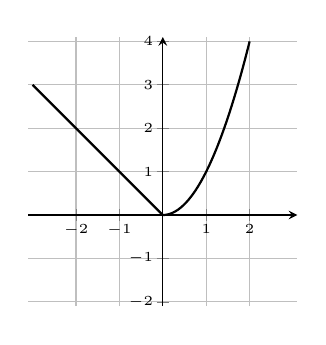
\begin{tikzpicture}%[domain=-4:4]
    \begin{axis}[
    grid=major,
    axis x line = middle,
    axis y line = middle,
        yticklabel style = {font=\tiny,xshift=0.5ex},
        xticklabel style = {font=\tiny,yshift=0.5ex},
    %scale only axis=true,
    width=5 cm,
    height=5 cm,
    xtick={-2,-1,0,1,2},
    ytick={-2,-1,0,1,2,3,4},
    xmin=-3.1,
    xmax=3.1,
    ymin=-2.1,
    ymax=4.1,
    ]
\addplot[smooth, thick, domain = 0:2,samples=35] { (x^2)};
\addplot[smooth, thick, domain = -3:0,samples=35] { -x};
  \end{axis}
\end{tikzpicture}

\choice \phantom{a}\vspace{-.7cm}
    
    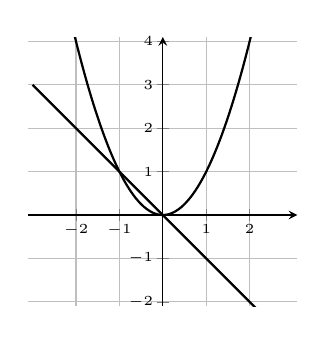
\begin{tikzpicture}%[domain=-4:4]
    \begin{axis}[
    grid=major,
    axis x line = middle,
    axis y line = middle,
        yticklabel style = {font=\tiny,xshift=0.5ex},
        xticklabel style = {font=\tiny,yshift=0.5ex},
    %scale only axis=true,
    width=5 cm,
    height=5 cm,
    xtick={-2,-1,0,1,2},
    ytick={-2,-1,0,1,2,3,4},
    xmin=-3.1,
    xmax=3.1,
    ymin=-2.1,
    ymax=4.1,
    ]
\addplot[smooth, thick, domain = -2.1:2.1,samples=35] { (x^2)};
\addplot[smooth, thick, domain = -3:3,samples=35] { -x};
  \end{axis}
\end{tikzpicture}
\choice \phantom{a}\vspace{-.7cm}
    
    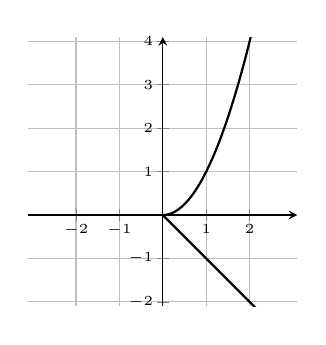
\begin{tikzpicture}
    \begin{axis}[
    grid=major,
    axis x line = middle,
    axis y line = middle,
        yticklabel style = {font=\tiny,xshift=0.5ex},
        xticklabel style = {font=\tiny,yshift=0.5ex},
    width=5 cm,
    height=5 cm,
    xtick={-2,-1,0,1,2},
    ytick={-2,-1,0,1,2,3,4},
    xmin=-3.1,
    xmax=3.1,
    ymin=-2.1,
    ymax=4.1,
    ]

\addplot[smooth, thick, domain = 0:2.1,samples=35] { (x^2)};
\addplot[smooth, thick, domain = 0:3,samples=35] { -x};
  \end{axis}
\end{tikzpicture}

\end{checkboxes}
\end{multicols}

\question[3] If $f(x)=3x^2-\dfrac{5}{2-x}$, What is $f(-2x)$?
\begin{checkboxes}
    \choice $12x^2-\dfrac{5}{2+2x}$
    \choice $-6x^3+\dfrac{10x}{2-x} $
    \choice $-6x^3-\dfrac{5}{2+2x}$
    \choice $-12x^2+\dfrac{5}{2-2x}$
    \choice None of the above.
\end{checkboxes}

\newpage
\question[3] Estimate the range of $f(x)$ for the graph shown below:

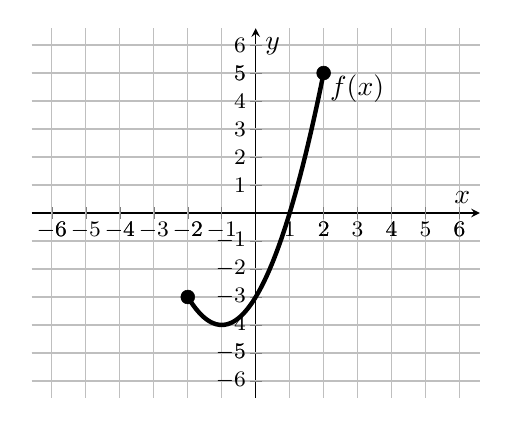
\begin{tikzpicture}
\begin{axis}[
   grid = major,
   extra x ticks={-6,-5,-4,-3,-2,-1,1,2,3,4,5,6},
   extra y ticks={-6,-5,-4,-3,-2,-1,1,2,3,4,5,6},
   %xminorgrids=true,
   width=.6\textwidth,
   %clip = true,
   %clip mode=individual,
   %restrict y to domain=-12:12,
   axis x line = middle,
   axis y line = middle,
        yticklabel style = {font=\footnotesize,xshift=0.5ex},
        xticklabel style = {font=\footnotesize,yshift=0.5ex},
   xlabel={$x$},
   %xlabel style={at=(current axis.right of origin)},
   ylabel={$y$},
   %ylabel style={at=(current axis.above origin)},
   %domain = -5:5,
   xmin = -6,
   xmax = 6,
   enlarge y limits={rel=0.05},
   enlarge x limits={rel=0.05},
   ymin = -6,
   ymax = 6,
 ]
\addplot[smooth, ultra thick, domain = -2:2,samples=35
	] { (x^2+2*x)-3}
 node[pos=.95](endofplotsquare){} ;
\node [right] at (endofplotsquare) {$f(x)$};%
        \addplot[only marks,mark=*, line width=0.2pt, mark size=2.5pt] coordinates{(-2,-3)(2,5) };
\end{axis}
\end{tikzpicture}
\begin{checkboxes}
    \choice $[-2,2]$
    \choice $[-3,5]$
    \choice $[-4,5]$
    \choice $[-2,5]$
    \choice None of the above.
\end{checkboxes}

\question[3] %Ang Complex number
%Simplify the following to a real number.
%\[(i^5+1)^2-2i\]
Solve the following quadratic equation:\\
\[x^2+4=0\]
\begin{checkboxes}
    \choice $x=-4$
    \choice $x=2$
    \choice $x=2$ or $x=-2$
    \choice $x=2i$ or $x=-2i$
    \choice The equation has no solution.
\end{checkboxes}

\newpage
\hspace{-.5in}Free answer section. Work must be shown to get credit for any answer. Partial credit may be given even for incorrect final answers, so show your work.

\question[5] %Factoring Question by John Yin Factor 
Factor the following quadratic. (Note: do not solve for this problem.)
\[
3x^2+17x-6
\]
\vfill


\question[6] Perform the following operation and simplify. Your final answer should be
written as a single fraction and contain no common factors in the numerator and
denominator.

\[
\frac{3}{2x^2+x-6} + \frac{1}{x+2}
\]
\vfill
\newpage

\question Given two points $A(2,7)$ and $B(6,5)$.
\begin{parts}
    \part[2] Find the midpoint of $A$ and $B$.
    \vspace{3cm}
    \part[2] Find the slope of the line through $A$ and $B$.
    \vspace{4cm}
    \part[3] Find the equation of the line through $A$ and $B$.
    \vspace{4cm}
    \part[3] Find the equation of the line through $(-3,1)$ perpendicular to the line through $A$ and $B$.
\end{parts}

\newpage



\question
\begin{parts}
    \part[6] Find \underline{all} solutions to the equation $x^4-1=0$. \\
    (Hint: Let $y=x^2$ and solve for $y$ first).
    \vfill
    \part[4] Find all solutions to the equation $x^5=x$. \\
    (Hint: Can you use anything from part (a)?)
    \vfill
\end{parts}

\question[6]
Solve for $x$: 
\[3x^2 -7x-2=-2x\]
\vfill

\newpage

%Logan Inequalities

\question Solve each of the following inequalities. {For each part, express your answer in interval notation and then graph it on a number line.}
\begin{parts}
    \part[5] $3\le-3x+2$
    \vspace{5cm}
    \part[5] $-11\le3x-5<10$
    \vspace{5cm}
    \part[6] $-x^2\ge-7x+10$
    \vspace{5cm}
\end{parts}
\newpage
%John S Absolute Value
\question[6] Find the possible value(s) for $x$ if $$4|x+3|-1 = 7.$$

\vfill
\question[6] For the function $f(x)=\sqrt{x^2-4}$, find the domain of $f(x)$. Write your answers in interval notation.

\vfill
\newpage



\question Find the \underline{average rate of change} for the functions below on the indicated intervals.
\begin{parts}
    \part[4] $f(x) = x^2+5x+8$ on $[-1,3]$.
    \vspace{9cm}
    \part[4] $g(x) = \dfrac{6}{1+x^3}$ on $[0,2]$.
    \vspace{5cm}
\end{parts}
\newpage

\question Solve the following equations.% for all solutions. %[Note 1: At least one of the following will have no solution. For that one, write that is has no solution.] (Note 2: there may be more than one solution, and the solutions may be complex).
\begin{parts}

	\part[6] 
	$  \dfrac{1-x}{x+2}=-3 $

\vfill	

% 	\part[5] 
% 	$  2x^2+x-10=0 $

% \vfill
	

	\part[6] $  \sqrt{6-x}=-x $

\vfill	

\end{parts}
\end{questions}